\chapter{Pilottest}
\label{TestAfSkalaPilottest}
%
(Der udføres én eller flere pilottest på AAU, som beskrives og evalueres i dette kapitel)

\textbf{Første pilottest}: PDP'er mand 25 (Svarer på skalaerne på papir)\\

Kommenterede at robotten kom lidt for tæt på, så han rykkede et stridt tilbage (robotten skulle komme tæt på)\\

OBS: Hver opmærksom på ordvalg - parametre, interaktion, ikke "ked af at sige det", ikke grin af besvarelserne de skal ikke føle sig overvåget.\\ 

I tvivl om det første spørgsmål - hvordan synes du skærmen reagerede - er i tvivl om hvorvidt det handler om hvordan det var at trykke på skærmen eller om det handlede om de valgmuligheder, der blev præsenteret var tilfredsstillende. (måske skriv spørgsmålet: Hvordan synes du skærmen reagerede på robotten, når du trykkede?)\\ 

I tvivl om hvad anmassende betyder - den kørte sådan lidt ind i mig i starten er det sådan noget? Får af vide at det er hvordan han forstår det. Er i tvivl om at forstå ordet "anmassende", jeg kunne se det som om at robotten presser sig på, da jeg stod derude kørte den sådan lidt hen til mig og ind i mig. Hvis robotten blev ved ville jeg føle at den var ret anmassende men efter noget tid holdte den afstand og så var den egentlig ikke anmassende.\\

Sjov - er meget subjektiv, han synes ikke den var sjov sjov (hahaha sjov) - træk ikke på smilebåndet. 

\textbf{Anden pilottest:} Vejleder kvinde (OBS: bliver gjort på samme skalaer med markeringer som første pilottest - papir). Markerer med en stjerne.\\

Har mange problemer med skærmen til at starte med.\\

Drop "ked af at sige"\\ 

Bedre at sige: "du har lige snakket med den her robot og jeg vil gerne vide lidt om din oplevelse..."\\

OBS: Overvej hvor skalaerne skal besvares henne - siddende, stående..\\

OBS: Behøver ikke at nævne hvor mange skalaer, 24 lyder at meget og kan være svært at forholde sig til.\\ 

I tvivl om hvad der menes med personlig (i forbindelse med personlig hjælp) - i forhold til mig?.\\ 

Kommenterer at "hvad synes du om robotten" kommer to gange - det må nok være det samme. På anden side kan man bruge overskriften "Synes du robotten er" eller "hvad synes du ellers om robotten", så man ikke får det samme, der kan man blive i tvivl om man skal svare på det samme igen. \\

Overvej spørgsmålet "Hvad er din kendskab til teknologi" - det er meget abstrakt og kan være svært at forholde sig til. Man kan spørger "Er du glad for teknologi?" - Spørg måske ind til om de synes det er let at bruge sin telefon eller computer. Har du en smartphone, hvornår har du sidst skiftet. \\ 

OBS: Til den forrige undersøgelse kunne vi have observeret folks reaktion på at robotten kører lidt tilbage når den bliver skubbet til og så derefter kommer tilbage.\\

OBS: Overvej om vi skal skrive på skærmen at man ikke skal trykke hårdt.  Der bliver tilføjet "(Tryk blidt på mig) på det første skærmbillede.\\

OBS: Både teknologi spørgsmålet og hvor mange gange man flyver på et år er ændret. \\

\textbf{Pilottest tre}: Mand 25 pdp'er\\
Ikke nævn hvor mange skalaer der er! eller at tiden afhænger af hvor hurtig man er.\\

Ikke stå bag ved og kig på hvad TP trykker på\\

Oplever problemer med skærmen

Jeg føler mig tryg ved robottens - OBS: Tjek at skalaerne i programmet er stavet rigtigt!


\section{Ændringer til pilottest}

%
\begin{figure}[H]
\centering
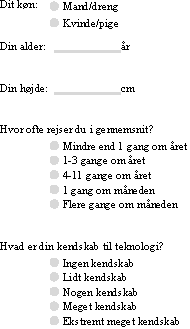
\includegraphics[width = 0.5\textwidth]{Figure/TestdesignEvaluering/Demografi} 
\caption{Ny.}
\label{fig:Demografi}
\end{figure}
\noindent
%

%
\begin{figure}[H]
\centering
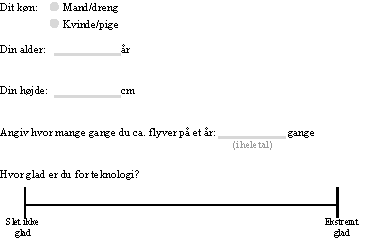
\includegraphics[width = 0.9\textwidth]{Figure/TestdesignEvaluering/TilpassetDemografi} 
\caption{Ny.}
\label{fig:TilpassetDemografi}
\end{figure}
\noindent
%

%
\begin{figure}[H]
\centering
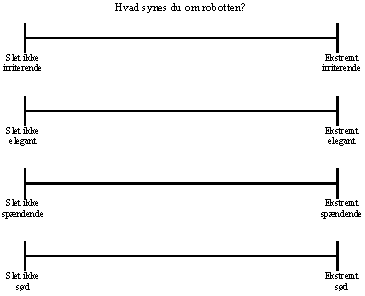
\includegraphics[width = 0.9\textwidth]{Figure/TilpasningAfSkalaer/TilpassetHvadSynesDuOmR} 
\caption{Ny.}
\label{fig:TilpassetHvadSynesDuOmR}
\end{figure}
\noindent
%

%
\begin{figure}[H]
\centering
\includegraphics[width = 0.9\textwidth]{Figure/TilpasningAfSkalaer/TilpassetHvadSynesDuEllersOmR} 
\caption{Ny.}
\label{fig:TilpassetHvadSynesDuEllersOmR}
\end{figure}
\noindent
%
 